\chapter{Clustering}  \label{clustering}
In Chapter~\ref{ch4}, I proposed an algorithm to construct an anti-unifier from the AUASTs of a pair of LMs, paying special attention to log statements. Recall that the general point of this study is to provide a description of where log statements happen in source code by constructing structural generalizations that represent the detailed commonalities and differences between the AUASTs of LMs. To this end, I require an algorithm that:
\begin{itemize} [leftmargin=.5in]
\item categorizes the methods showing different ways of locating log statements into separate clusters; and
\item abstracts the AUASTs of LMs of each group into a structural generalization representing the similarities and differences between them.
\end{itemize}

In Section~\ref{m-clustering-alg}, I describe a modified version of an agglomerative hierarchical clustering algorithm that I developed for my application. The clustering algorithm is a bottom-up approach that starts with singleton clusters, each containing one AUAST, and then it repeatedly merges the closest clusters that are the ones with maximum similarity between their AUASTs. To evaluate my approach, I have implemented the clustering tool and conducted an evaluation through the application of it on the test suite introduced in Section~\ref{study1_setup}. I describe my empirical study and discuss the results in Section~\ref{clustering-evaluation}.
% I developed for my application.?

%Therefore, before the use a clustering algorithm to classify a set of AUASTs, I need to first
%Clustering is the classification of a collection of unlabelled data items into meaningful groups \cite{jain1999data}, where category labels are obtained from the similarities between data items.


\section{Modified agglomerative hierarchical clustering algorithm} \label{m-clustering-alg}
%To develop a measure of similarity between AUASTs, I used the similarity function described in Section~\ref{meth-similarity}.
%unsupervised???
%by computing pairwise similarities between cluster pairs?
Clustering is an unsupervised machine learning technique that aims to organize a collection of data into clusters, such that intra-cluster similarity is maximized and the inter-cluster similarity is minimized \cite{karypis1999chameleon,grira2004unsupervised}.
To perform clustering on a set of AUASTs of LMs, I developed Algorithm~\ref{modified-agglomerative}, which is a modified version of the basic agglomerative hierarchical clustering algorithm described in Section~\ref{ch3-clustering}. The clustering algorithm is a bottom-up approach that starts with singleton clusters, each containing one AUAST (line~1), and then it creates a similarity matrix by computing pairwise similarities between cluster pairs (line~2). This step requires defining a notion of cluster similarity. As I aim to construct an anti-unifier for each cluster, the similarity between two clusters is measured based on the similarity between their AUASTs.
%\RW{Add to bib},
%\RW{Note: you don't describe this tool in any detail.  I am assuming it is straightforward.}\NZ{ Yes, It is straightforward. I just implemented the algorithm I described here.}
%\RW{Why did you do it manually?  You are assuming that your manual approach represents the ground truth, which may not be true; this is a point for discussion in threats to validity.}\NZ{ I changed the way I evaluated the clustering algorithm, and defined some measurements that can be calculated using equations.}



In general, this hierarchical algorithm employs an $n \times n$ similarity matrix for a set of $n$ AUASTs, where an element in row $i$ and column $j$ represents the similarity between the $i$th and the $j$th clusters. The similarity between two clusters is defined as the similarity between their AUASTs, which is computed through the algorithm described in Section~\ref{meth-similarity}. However, there are some cases in which the anti-unification of the AUASTs of two clusters does not allow the anti-unification of log statements with one another, since the structures enclosing them are not corresponded. To handle these cases, I adjusted the similarity value between the two clusters to zero. Then the algorithm repeatedly merges the closest clusters that are the ones with maximum similarity between their AUASTs, and updates the similarity matrix by computing the similarity between the new cluster and the old ones (lines~5--6). The merge and update steps are repeated until the similarity between closest clusters becomes below a predetermined threshold value (line~7). Through informal examination, I have found that a threshold value of 0.05 gives the reasonable results, as it allows the classification of methods showing different ways of locating log statements in separate clusters. I also used the anti-unification algorithm described in Section~\ref{meth-antiUnifier} to construct an anti-unifier for each cluster.
%threshold???
%allows? the classification of methods showing different ways of locating log statements in separate clusters?

 %to prevent the combination of a cluster pair when the usage of logging is different, I adjusted the similarity between them to zero. they should be in separate clusters.


\begin{algorithm}
\caption{Modified agglomerative hierarchical clustering algorithm.} \label{modified-agglomerative}
\begin{algorithmic}[1]
\State Start with singleton clusters.
\State Compute a similarity matrix.
\Repeat
\State Find the closest clusters.
\State Merge the closest cluster pair and replace the original clusters with a new one containing the anti-unifier of their AUASTs.
\State Update the similarity matrix by computing the similarity between new cluster and all remaining clusters.
\Until the similarity between closest clusters becomes below a predetermined threshold value.
\end{algorithmic}
\end{algorithm}


A hierarchical clustering algorithm can be displayed using a tree-like diagram that shows the order in which the clusters were merged. For example, Figure~\ref{fig:overview2} illustrates the modified agglomerative hierarchical clustering process for a sample set of 3 AUASTs using the initial similarity matrix depicted in Figure~\ref{matrix}. It starts with all AUASTs as singleton clusters. In the first iteration, clusters~\#1 and~\#2 are selected as the closest clusters, they are then merged and replaced by cluster~\#4. If the threshold value is set at 0.20, the process should be terminated at this step, as the similarity between the closest clusters (clusters~\#3 and~\#4) is below this threshold; otherwise, these clusters should be merged and replaced by cluster~\#5.


 %The threshold value indicates the number of resulting clusters.
%the relationship between clusters and subclusters, and


%However, the similarity between AUASTs of clusters 7 and 8 is zero, and thus they should not be merged with each other.
%THRESHOLD B??

\begin{figure}[h]
  \centering
    \centering
   \begin{displaymath}
    similarity = \left[
        \begin{matrix}
        1.00 &  &     \\
0.48 & 1.00 &    \\
0.12 & 0.17 & 1.0   \\
        \end{matrix}   \right]
\end{displaymath}
 \caption{The initial similarity matrix for a sample set of 3 AUASTs.}
  \label{matrix}
  \end{figure}

  \begin{figure} [h]

   \centering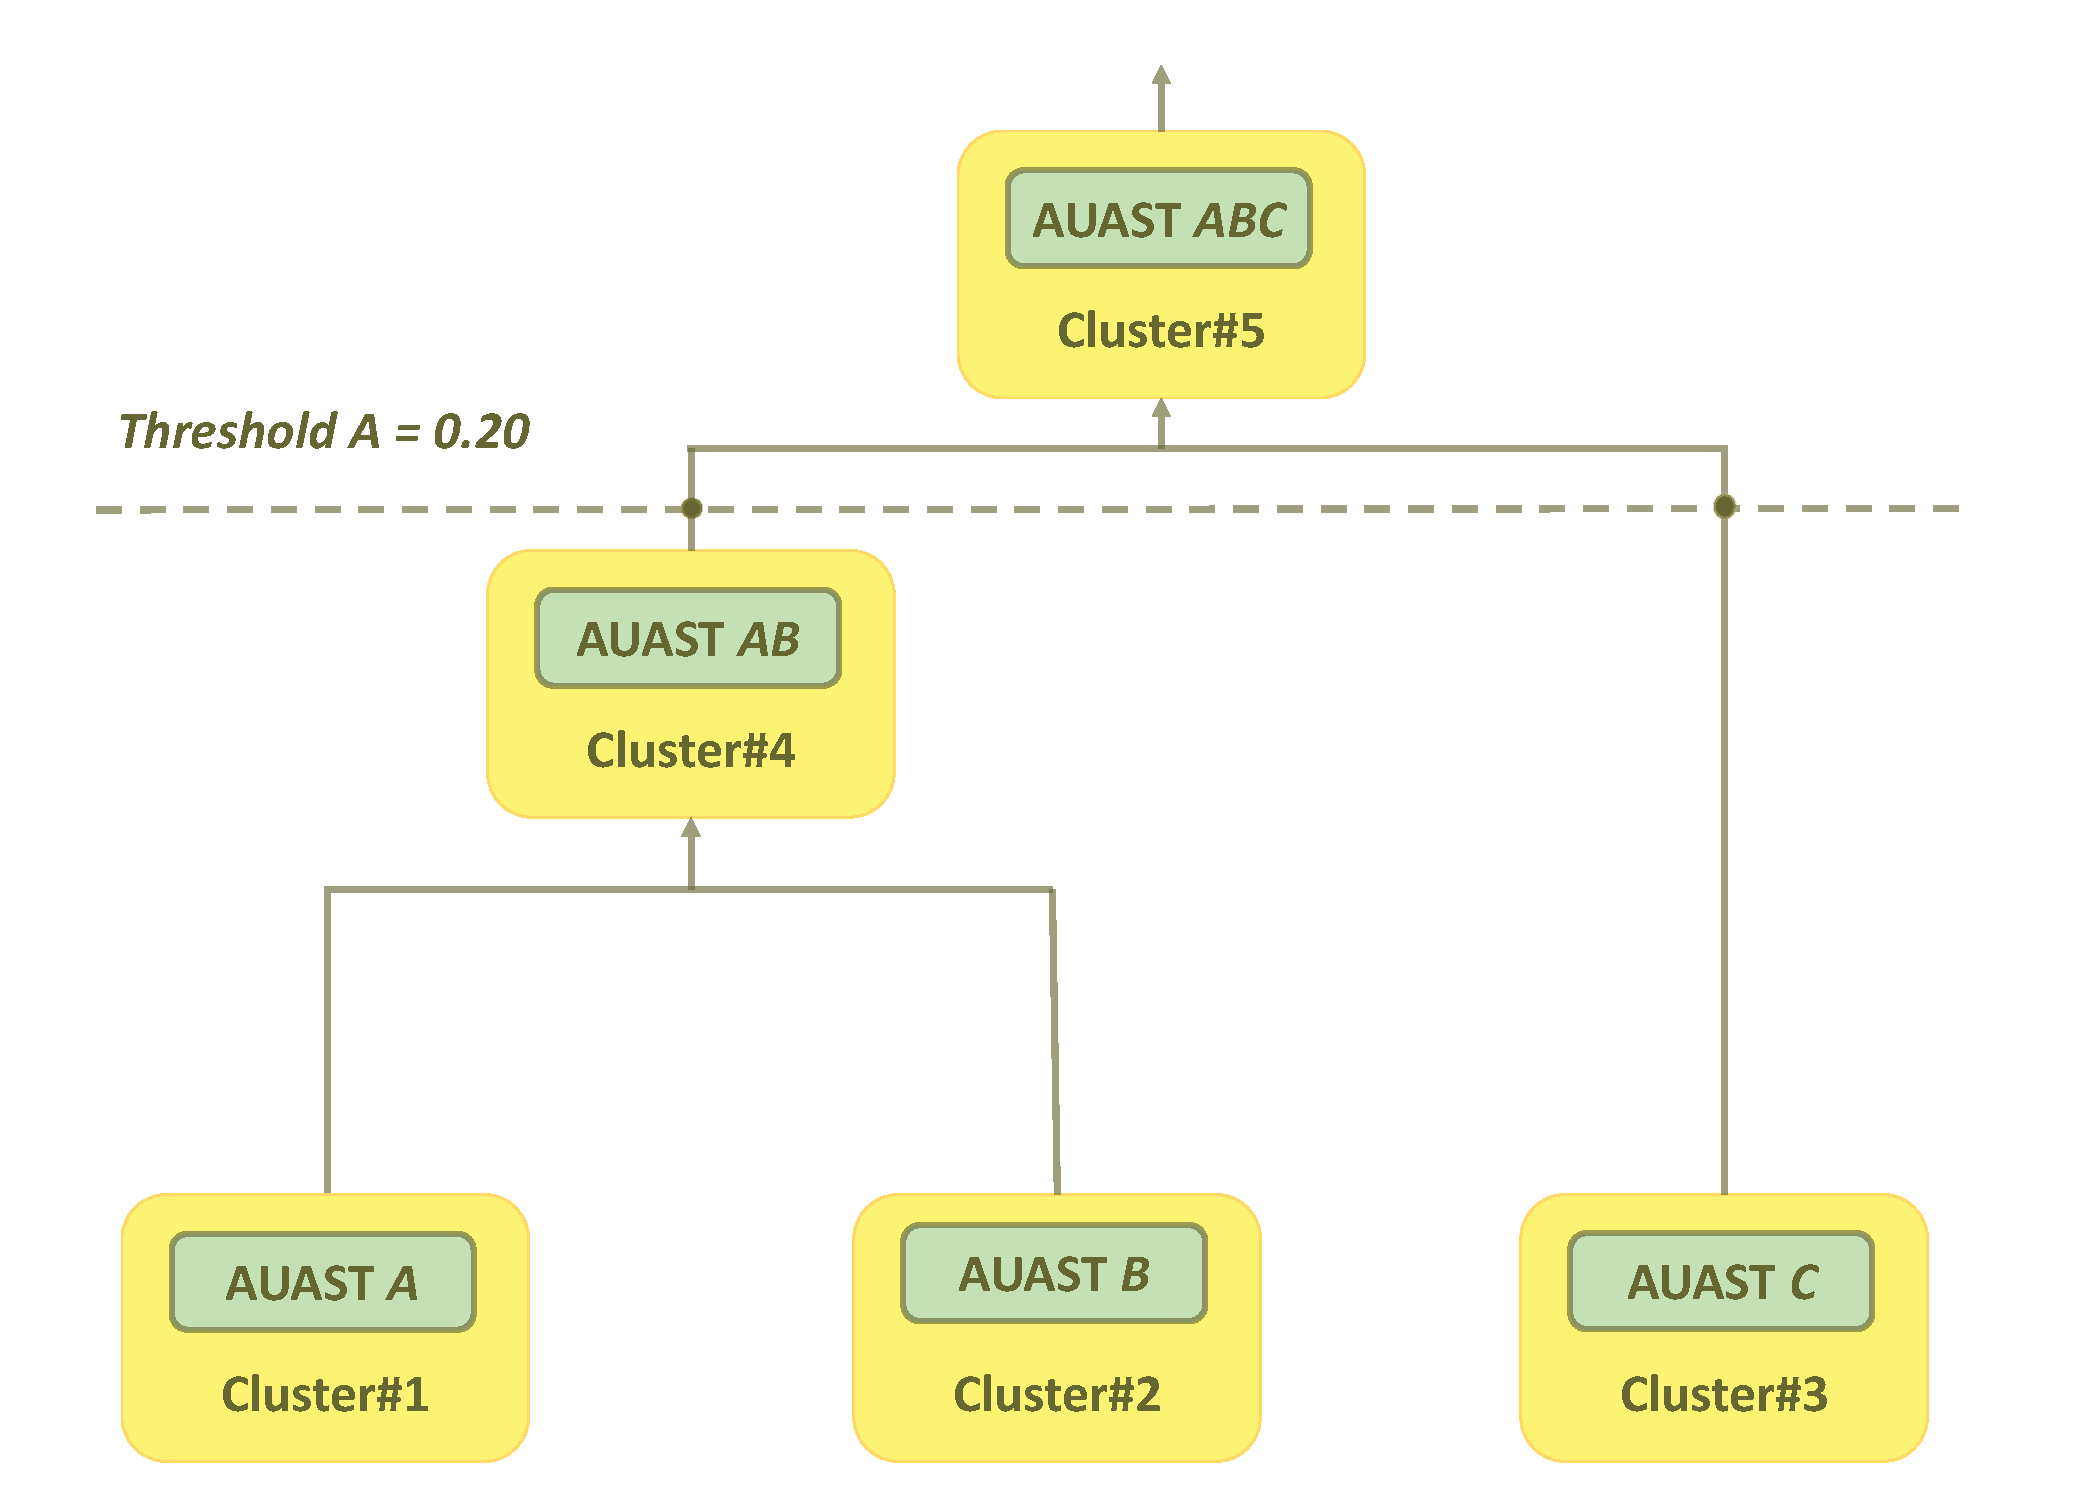
\includegraphics [width = 0.8\textwidth]{Drawing4/clustering.pdf}
  \caption{Diagram of the modified agglomerative hierarchical clustering process for the sample set.}
  \label{fig:overview2}
\end{figure}
%caption???
% \caption{The similarity matrix for a sample set of 3 AUASTs.}
 % \caption{The modified agglomerative hierarchical clustering process on a sample set of 3 AUASTs using the initial similarity matrix shown in Figure~\ref{matrix}. The threshold value indicates the number of resulting clusters.}


%\section{An assessment of the Clustering tool} \label{clustering-assessment}
%To evaluate the quality of a clustering algorithm
\section{Evaluation} \label{clustering-evaluation}
To evaluate the clustering approach, I have implemented a tool and conducted an experiment on the set of AUASTs of LMs described in Table~\ref{table:ljms}. The clustering tool is an Eclipse plug-in built atop the anti-unifier building tool that inputs a set of AUASTs of LMs extracted from the source code, applies the clustering algorithm on them, and outputs an anti-unifier for each cluster. Then, I have developed some measurements to assess the goodness of the resulting clusters. Recall that clustering should be performed in such a way that the objects within a cluster are similar to one another and dissimilar from the other clusters \cite{tan2005data}. The measures of cluster evaluation can be divided into two types:

%. Recall that clustering should be performed in such a way that the objects within a cluster are similar to one another and dissimilar from the other clusters \cite{tan2013data} ?
\begin{itemize} [leftmargin=0.4in]
\item \emph{Cluster cohesion:} which determines how closely related the objects within a cluster are. In this experiment, the cohesion of each cluster can be defined as the average of the similarities between the AUAST pairs in each cluster.
\item \emph{Cluster separateness:} which determines how distinct or well-separated a cluster is from the other clusters. A well-separated cluster is a set of data objects in which each object is more similar to every other object in the cluster than to any other object in the other clusters.  In this experiment, the separation between two clusters can be measured by the similarity between the two clusters anti-unifiers (representatives). 
\end{itemize}
% and the AUAST of the cluster anti-unifier
%\subsection{Setup}  \label{study3-setup}
%I manually attempted to perform the hierarchical clustering on the set AUASTs of LMs in the test suite and constructed the detailed anti-unifier view for each cluster. Anti-unifiers were discarded when the anti-unification of LMs did not allow the anti-unification of logging calls with one another, as the Java elements enclosing them were not found to be corresponded. I also measured the level of similarity between AUASTs in each cluster by computing the ratio of common Java elements in the detailed anti-unifier view to the total number of Java elements of all AUASTs in that cluster. I also ran the clustering tool on the set of AUASTs to classify them using the similarity measurement.

%using the following equations, respectively:

%\begin{equation}
%separateness(C_i,C_j) = similarity(antiUnifier[C_i],antiUnifier[C_j])
%\end{equation}

%\begin{equation}
%cohesion(C_i) = \frac{ \sum_{x \in C_i}  similarity(x,antiUnifier[C_i] )}{(N_i*N_i+1)\2}
%\end{equation}


%\begin{equation}
%cohesion(C_i) = \frac{ \sum_{x \in C_i}  similarity(x,antiUnifier[C_i] )}{N_i}
%\end{equation}



\subsection{Results}  \label{study3-results}

%I present the results of my analysis in Table~\ref{results_clustering}. The analysis of the output has been divided into three categories: correspondence, similarity, and separateness. The analysis of correspondence and similarity was described in Section~\ref{study2-results}. "Separateness" refers to my tools' ability to cluster Java method with different usages of log statements into separate groups, and the ones with similar usages of log statements into the same cluster.
%To evaluate the quality of the resulting clusters, I computed the cohesion of each cluster and the separateness between each cluster pair

I ran the clustering tool on the set of AUASTs of the test suite described in Table~\ref{table:ljms}. The cohesion of the clusters produced by applying the clustering tool to the test suite is presented in Table~\ref{tab:cohesion}, where $C_i$ is the  $i$th cluster, and $N_i$ is the cluster size of cluster ${C_i}$. In addition, Table~\ref{tab:separateness} shows the separateness between each cluster pair. 
%\RW{What is separateness? The table shows straight zeroes.  What does this mean?}
%\NZ{Separateness measures  how distinct or well-separated a cluster is from the other clusters. A well-separated cluster is a set of data objects in which each object is more similar to every other object in the cluster than to any other object in the other clusters. In this experiment, the separation between two clusters can be measured by the similarity between the two clusters anti-unifiers, which are representatives of the clusters.
%As I explained in Section~\ref{{m-clustering-alg}}, I adjusted the similarity to zero to handle the cases in which the anti-unification of the AUASTs of two clusters does not allow the anti-unification of log statements with one another, since the structures enclosing them are not corresponded. This is the reason why I got straight zero. This results implies that that logged methods in each cluster should be located in that cluster and not the other clusters.}


%The cohesion of the clusters produced by applying the clustering tool to the test suite described in Table~\ref{table:ljms}

%The separateness between each cluster pair produced by applying the clustering tool to the test suite described in Table~\ref{table:ljms}
\begin{minipage}[b]{.40\textwidth}
   \centering
   \begin{tabular}{ ccc}\toprule
     {Cluster}&{$N_i$}&{Cohesion}\\
    \toprule
    $C_1$&4& 0.26 \\
    \midrule
    $C_2$&3& 0.40\\
    \midrule
    $C_3$&3& 0.32\\
 	\bottomrule
   \end{tabular}
   \captionof{table}{The cohesion of clusters.}
   \label{tab:cohesion}
\end{minipage}\qquad
\begin{minipage}[b]{.40\textwidth}
   \centering
   \begin{tabular}{ cc}\toprule
     {Cluster}&{Separateness}\\
    \toprule
    $C_1$--$C_2$& 0\\
    \midrule
    $C_1$--$C_3$& 0\\
    \midrule
    $C_2$--$C_3$& 0\\
 	\bottomrule
   \end{tabular}
   \captionof{table}{The separateness of clusters.}
   \label{tab:separateness}

   %\caption{The separateness of the resulting cluster pairs.}
\end{minipage}

%        \caption{The cohesion and separateness of the resulting clusters.}

% of the test suite described in Table~\ref{table:ljms}
Clusters $C_1$, $C_2$, and $C_3$ contain logged methods of cases 1, 3, 5, and 8; cases 2, 9, and 10; and cases 4, 6, and 7; respectively.
The separation results show that my algorithm was able to generate well-separated clusters.
As I explained in Section~\ref{m-clustering-alg}, I adjusted the similarity to zero to handle the cases in which the anti-unification of AUASTs of LMs does not allow the anti-unification of log statements with one another, which is the reason behind the separateness of zero between the resulting cluster pairs. The separateness results also imply that logged methods in each cluster should be located in that cluster and not the other ones. The cohesion results show that all LMs in the same cluster are related to one another. In general, this experiment shows that my algorithm results in good quality clusters in terms of cohesion and separateness measurements.
%the resulting clusters which indicates that the
%, as detected by my manual inspection.
%, as the LMs within each cluster used similar ways of locating log statements and dissimilar ways compared to the other Lms in the other clusters.


%?????
%The clustering tool succeeded in detecting the separateness amongst AUASTs of test cases correctly. Clusters 1, 2, and 3 contain logged methods of cases (1, 3, 5, 8), (4, 6, 7), and (2, 9, 10), respectively, as detected by my manual inspection. It also successfully calculated the similarity between LMs of 2 clusters out of 3. In Cluster 2, the error in detecting correspondences originated from the previous study and propagated to the clustering study. However, it is trivial (0.01) and would have a low impact on our final results.
%between the LMs of our test suite.

\section{Summary} \label{meth2-summary}
I have presented a modified version of the agglomerative hierarchical clustering algorithm to categorize logged methods showing different usages of log statements into separate clusters. This algorithm is implemented as an Eclipse plug-in that takes a set of AUASTs of LMs, clusters them into separate groups, and generates an anti-unifier for each cluster. Furthermore, an experimental study was conducted to validate the effectiveness of my clustering algorithm and the tool support on a test suite.




